% Options for packages loaded elsewhere
\PassOptionsToPackage{unicode}{hyperref}
\PassOptionsToPackage{hyphens}{url}
%
\documentclass[
]{book}
\usepackage{lmodern}
\usepackage{amssymb,amsmath}
\usepackage{ifxetex,ifluatex}
\ifnum 0\ifxetex 1\fi\ifluatex 1\fi=0 % if pdftex
  \usepackage[T1]{fontenc}
  \usepackage[utf8]{inputenc}
  \usepackage{textcomp} % provide euro and other symbols
\else % if luatex or xetex
  \usepackage{unicode-math}
  \defaultfontfeatures{Scale=MatchLowercase}
  \defaultfontfeatures[\rmfamily]{Ligatures=TeX,Scale=1}
\fi
% Use upquote if available, for straight quotes in verbatim environments
\IfFileExists{upquote.sty}{\usepackage{upquote}}{}
\IfFileExists{microtype.sty}{% use microtype if available
  \usepackage[]{microtype}
  \UseMicrotypeSet[protrusion]{basicmath} % disable protrusion for tt fonts
}{}
\makeatletter
\@ifundefined{KOMAClassName}{% if non-KOMA class
  \IfFileExists{parskip.sty}{%
    \usepackage{parskip}
  }{% else
    \setlength{\parindent}{0pt}
    \setlength{\parskip}{6pt plus 2pt minus 1pt}}
}{% if KOMA class
  \KOMAoptions{parskip=half}}
\makeatother
\usepackage{xcolor}
\IfFileExists{xurl.sty}{\usepackage{xurl}}{} % add URL line breaks if available
\IfFileExists{bookmark.sty}{\usepackage{bookmark}}{\usepackage{hyperref}}
\hypersetup{
  pdftitle={Introdução ao R},
  pdfauthor={Raimundo Marciano de Freitas Neto},
  hidelinks,
  pdfcreator={LaTeX via pandoc}}
\urlstyle{same} % disable monospaced font for URLs
\usepackage{color}
\usepackage{fancyvrb}
\newcommand{\VerbBar}{|}
\newcommand{\VERB}{\Verb[commandchars=\\\{\}]}
\DefineVerbatimEnvironment{Highlighting}{Verbatim}{commandchars=\\\{\}}
% Add ',fontsize=\small' for more characters per line
\usepackage{framed}
\definecolor{shadecolor}{RGB}{248,248,248}
\newenvironment{Shaded}{\begin{snugshade}}{\end{snugshade}}
\newcommand{\AlertTok}[1]{\textcolor[rgb]{0.94,0.16,0.16}{#1}}
\newcommand{\AnnotationTok}[1]{\textcolor[rgb]{0.56,0.35,0.01}{\textbf{\textit{#1}}}}
\newcommand{\AttributeTok}[1]{\textcolor[rgb]{0.77,0.63,0.00}{#1}}
\newcommand{\BaseNTok}[1]{\textcolor[rgb]{0.00,0.00,0.81}{#1}}
\newcommand{\BuiltInTok}[1]{#1}
\newcommand{\CharTok}[1]{\textcolor[rgb]{0.31,0.60,0.02}{#1}}
\newcommand{\CommentTok}[1]{\textcolor[rgb]{0.56,0.35,0.01}{\textit{#1}}}
\newcommand{\CommentVarTok}[1]{\textcolor[rgb]{0.56,0.35,0.01}{\textbf{\textit{#1}}}}
\newcommand{\ConstantTok}[1]{\textcolor[rgb]{0.00,0.00,0.00}{#1}}
\newcommand{\ControlFlowTok}[1]{\textcolor[rgb]{0.13,0.29,0.53}{\textbf{#1}}}
\newcommand{\DataTypeTok}[1]{\textcolor[rgb]{0.13,0.29,0.53}{#1}}
\newcommand{\DecValTok}[1]{\textcolor[rgb]{0.00,0.00,0.81}{#1}}
\newcommand{\DocumentationTok}[1]{\textcolor[rgb]{0.56,0.35,0.01}{\textbf{\textit{#1}}}}
\newcommand{\ErrorTok}[1]{\textcolor[rgb]{0.64,0.00,0.00}{\textbf{#1}}}
\newcommand{\ExtensionTok}[1]{#1}
\newcommand{\FloatTok}[1]{\textcolor[rgb]{0.00,0.00,0.81}{#1}}
\newcommand{\FunctionTok}[1]{\textcolor[rgb]{0.00,0.00,0.00}{#1}}
\newcommand{\ImportTok}[1]{#1}
\newcommand{\InformationTok}[1]{\textcolor[rgb]{0.56,0.35,0.01}{\textbf{\textit{#1}}}}
\newcommand{\KeywordTok}[1]{\textcolor[rgb]{0.13,0.29,0.53}{\textbf{#1}}}
\newcommand{\NormalTok}[1]{#1}
\newcommand{\OperatorTok}[1]{\textcolor[rgb]{0.81,0.36,0.00}{\textbf{#1}}}
\newcommand{\OtherTok}[1]{\textcolor[rgb]{0.56,0.35,0.01}{#1}}
\newcommand{\PreprocessorTok}[1]{\textcolor[rgb]{0.56,0.35,0.01}{\textit{#1}}}
\newcommand{\RegionMarkerTok}[1]{#1}
\newcommand{\SpecialCharTok}[1]{\textcolor[rgb]{0.00,0.00,0.00}{#1}}
\newcommand{\SpecialStringTok}[1]{\textcolor[rgb]{0.31,0.60,0.02}{#1}}
\newcommand{\StringTok}[1]{\textcolor[rgb]{0.31,0.60,0.02}{#1}}
\newcommand{\VariableTok}[1]{\textcolor[rgb]{0.00,0.00,0.00}{#1}}
\newcommand{\VerbatimStringTok}[1]{\textcolor[rgb]{0.31,0.60,0.02}{#1}}
\newcommand{\WarningTok}[1]{\textcolor[rgb]{0.56,0.35,0.01}{\textbf{\textit{#1}}}}
\usepackage{longtable,booktabs}
% Correct order of tables after \paragraph or \subparagraph
\usepackage{etoolbox}
\makeatletter
\patchcmd\longtable{\par}{\if@noskipsec\mbox{}\fi\par}{}{}
\makeatother
% Allow footnotes in longtable head/foot
\IfFileExists{footnotehyper.sty}{\usepackage{footnotehyper}}{\usepackage{footnote}}
\makesavenoteenv{longtable}
\usepackage{graphicx,grffile}
\makeatletter
\def\maxwidth{\ifdim\Gin@nat@width>\linewidth\linewidth\else\Gin@nat@width\fi}
\def\maxheight{\ifdim\Gin@nat@height>\textheight\textheight\else\Gin@nat@height\fi}
\makeatother
% Scale images if necessary, so that they will not overflow the page
% margins by default, and it is still possible to overwrite the defaults
% using explicit options in \includegraphics[width, height, ...]{}
\setkeys{Gin}{width=\maxwidth,height=\maxheight,keepaspectratio}
% Set default figure placement to htbp
\makeatletter
\def\fps@figure{htbp}
\makeatother
\setlength{\emergencystretch}{3em} % prevent overfull lines
\providecommand{\tightlist}{%
  \setlength{\itemsep}{0pt}\setlength{\parskip}{0pt}}
\setcounter{secnumdepth}{5}
\usepackage{booktabs}
\usepackage[]{natbib}
\bibliographystyle{apalike}

\title{Introdução ao R}
\author{Raimundo Marciano de Freitas Neto}
\date{2021-02-16}

\begin{document}
\maketitle

{
\setcounter{tocdepth}{1}
\tableofcontents
}
\hypertarget{prerequisites}{%
\chapter{Prerequisites}\label{prerequisites}}

This is a \emph{sample} book written in \textbf{Markdown}. You can use anything that Pandoc's Markdown supports, e.g., a math equation \(a^2 + b^2 = c^2\).

The \textbf{bookdown} package can be installed from CRAN or Github:

\begin{Shaded}
\begin{Highlighting}[]
\KeywordTok{install.packages}\NormalTok{(}\StringTok{"bookdown"}\NormalTok{)}
\CommentTok{# or the development version}
\CommentTok{# devtools::install_github("rstudio/bookdown")}
\end{Highlighting}
\end{Shaded}

Remember each Rmd file contains one and only one chapter, and a chapter is defined by the first-level heading \texttt{\#}.

To compile this example to PDF, you need XeLaTeX. You are recommended to install TinyTeX (which includes XeLaTeX): \url{https://yihui.org/tinytex/}.

\hypertarget{intro}{%
\chapter{O que é o R?}\label{intro}}

R é uma linguagem de programação muito utilizada para o desenvolvimento de estatísticas e cálculos matemáticos. Entretanto, enquanto linguagem de programação, ela possui muitos usos, como a raspagem de sites, a automatização de download de arquivos, e a produção de dashboards e relatórios, sendo útil para a coleta de dados e para o reporte das análises, além de ser gratuita.
Mas o que significa ser uma linguagem de programação? Basicamente, você irá dar ordens ao computador por meio de comandos. A vantagem de aprender a estruturar os comandos (ao invés de usar um programa estatístico já consolidado, como o Stata) é que você pode customizar a vontade suas análises. Os programas estatísticos trazem muitas opções pré-prontas. Por exemplo, no Stata é comum que você possa clicar em uma janela e solicitar um quadro com as estatísticas descritivas (média, moda, mediana) de um banco de dados. Entretanto, qualquer funcionalidade fora do padrão oferecido por aqueles pacotes precisará ser gerada pelo próprio usuário (e quando você usa algum recurso como o ssc install é porque alguém gastou um tempinho fazendo isso).

Aliás, o Python (outra linguagem de programação) possui funcionalidades bem similares ao R, embora o modo de escrever os programas seja bem diferente. Imagine que o Português e o Espanhol têm o mesmo propósito - a comunicação - e que mesmo tendo uma mesma raiz (e inclusive diversos vocábulos bem parecidos), possuem algumas regras estruturais bem diferentes, o que inclui, por exemplo, as regras de acentuação e o som produzidos pelas letras: qual a diferença de cajá (PT-BR) para caja (ES); qual a diferença de pastel (PT-BR) para pastel (ES)?

É preferível que o analista iniciante dedique-se a uma das duas (R ou Python). Posteriormente, aprender a outra (ou mais alguma que esteja despontando no mercado, como a Julia) será uma tarefa bem mais simples. Isso se deve ao fato de que diversos elementos da programação se repetem entre as diferentes linguagens, especialmente os conceitos. Um IF tem o mesmo propósito em R ou em Python ou em Java ou em C++, embora a forma como você deve explicar ao computador o que fazer com esse IF será bem diferente em cada linguagem.

You can label chapter and section titles using \texttt{\{\#label\}} after them, e.g., we can reference Chapter \ref{intro}. If you do not manually label them, there will be automatic labels anyway, e.g., Chapter \ref{methods}.

Figures and tables with captions will be placed in \texttt{figure} and \texttt{table} environments, respectively.

\begin{Shaded}
\begin{Highlighting}[]
\KeywordTok{par}\NormalTok{(}\DataTypeTok{mar =} \KeywordTok{c}\NormalTok{(}\DecValTok{4}\NormalTok{, }\DecValTok{4}\NormalTok{, }\FloatTok{.1}\NormalTok{, }\FloatTok{.1}\NormalTok{))}
\KeywordTok{plot}\NormalTok{(pressure, }\DataTypeTok{type =} \StringTok{'b'}\NormalTok{, }\DataTypeTok{pch =} \DecValTok{19}\NormalTok{)}
\end{Highlighting}
\end{Shaded}

\begin{figure}

{\centering 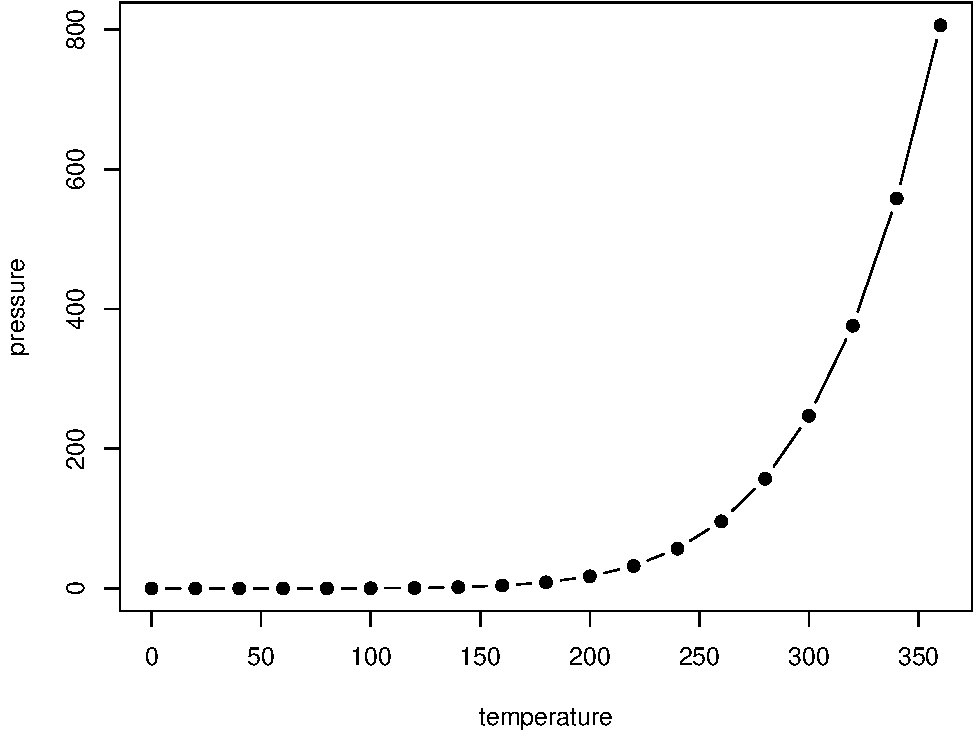
\includegraphics[width=0.8\linewidth]{introR_files/figure-latex/nice-fig-1} 

}

\caption{Here is a nice figure!}\label{fig:nice-fig}
\end{figure}

Reference a figure by its code chunk label with the \texttt{fig:} prefix, e.g., see Figure \ref{fig:nice-fig}. Similarly, you can reference tables generated from \texttt{knitr::kable()}, e.g., see Table \ref{tab:nice-tab}.

\begin{Shaded}
\begin{Highlighting}[]
\NormalTok{knitr}\OperatorTok{::}\KeywordTok{kable}\NormalTok{(}
  \KeywordTok{head}\NormalTok{(iris, }\DecValTok{20}\NormalTok{), }\DataTypeTok{caption =} \StringTok{'Here is a nice table!'}\NormalTok{,}
  \DataTypeTok{booktabs =} \OtherTok{TRUE}
\NormalTok{)}
\end{Highlighting}
\end{Shaded}

\begin{table}

\caption{\label{tab:nice-tab}Here is a nice table!}
\centering
\begin{tabular}[t]{rrrrl}
\toprule
Sepal.Length & Sepal.Width & Petal.Length & Petal.Width & Species\\
\midrule
5.1 & 3.5 & 1.4 & 0.2 & setosa\\
4.9 & 3.0 & 1.4 & 0.2 & setosa\\
4.7 & 3.2 & 1.3 & 0.2 & setosa\\
4.6 & 3.1 & 1.5 & 0.2 & setosa\\
5.0 & 3.6 & 1.4 & 0.2 & setosa\\
\addlinespace
5.4 & 3.9 & 1.7 & 0.4 & setosa\\
4.6 & 3.4 & 1.4 & 0.3 & setosa\\
5.0 & 3.4 & 1.5 & 0.2 & setosa\\
4.4 & 2.9 & 1.4 & 0.2 & setosa\\
4.9 & 3.1 & 1.5 & 0.1 & setosa\\
\addlinespace
5.4 & 3.7 & 1.5 & 0.2 & setosa\\
4.8 & 3.4 & 1.6 & 0.2 & setosa\\
4.8 & 3.0 & 1.4 & 0.1 & setosa\\
4.3 & 3.0 & 1.1 & 0.1 & setosa\\
5.8 & 4.0 & 1.2 & 0.2 & setosa\\
\addlinespace
5.7 & 4.4 & 1.5 & 0.4 & setosa\\
5.4 & 3.9 & 1.3 & 0.4 & setosa\\
5.1 & 3.5 & 1.4 & 0.3 & setosa\\
5.7 & 3.8 & 1.7 & 0.3 & setosa\\
5.1 & 3.8 & 1.5 & 0.3 & setosa\\
\bottomrule
\end{tabular}
\end{table}

You can write citations, too. For example, we are using the \textbf{bookdown} package \citep{R-bookdown} in this sample book, which was built on top of R Markdown and \textbf{knitr} \citep{xie2015}.

\hypertarget{scripts}{%
\section{Scripts}\label{scripts}}

\hypertarget{variuxe1veis}{%
\chapter{Variáveis}\label{variuxe1veis}}

Os dados são inseridos no R como variáveis. Eles podem ser importados (trazidos de um arquivo para o R) ou digitados no próprio console. Quando você deseja armazenar um valor na memória, você deve atribuí-lo, usando o sinal = ou \textless-.

\begin{Shaded}
\begin{Highlighting}[]
\NormalTok{x =}\StringTok{ }\DecValTok{1}
\KeywordTok{print}\NormalTok{(x)}
\end{Highlighting}
\end{Shaded}

\begin{verbatim}
## [1] 1
\end{verbatim}

\begin{Shaded}
\begin{Highlighting}[]
\NormalTok{y <-}\StringTok{ }\DecValTok{1}\OperatorTok{+}\DecValTok{1}
\NormalTok{y}
\end{Highlighting}
\end{Shaded}

\begin{verbatim}
## [1] 2
\end{verbatim}

\begin{Shaded}
\begin{Highlighting}[]
\NormalTok{texto =}\StringTok{ "Esse é um texto. Observe as aspas duplas"}
\NormalTok{assim =}\StringTok{ 'Também podem ser usadas aspas simples'}
\NormalTok{sugestao =}\StringTok{ 'Use aspas simples sempre que "possível" para delimitar a variável. Os }
\StringTok{textos em português costumam usadas aspas duplas.'}
\KeywordTok{print}\NormalTok{(sugestao)}
\end{Highlighting}
\end{Shaded}

\begin{verbatim}
## [1] "Use aspas simples sempre que \"possível\" para delimitar a variável. Os \ntextos em português costumam usadas aspas duplas."
\end{verbatim}

\begin{Shaded}
\begin{Highlighting}[]
\KeywordTok{writeLines}\NormalTok{(sugestao)}
\end{Highlighting}
\end{Shaded}

\begin{verbatim}
## Use aspas simples sempre que "possível" para delimitar a variável. Os 
## textos em português costumam usadas aspas duplas.
\end{verbatim}

O R é uma linguagem que automaticamente reconhece o tipo do dado que foi inserido. Por uma questão de comparação, se você estivesse usando uma linguagem \emph{tipada}, como o C++, você precisaria declarar explicitamente o tipo da variável que está sendo criada. Assim, seria um erro você criar uma variável usando

\begin{Shaded}
\begin{Highlighting}[]
\NormalTok{dois =}\StringTok{ }\DecValTok{2}
\end{Highlighting}
\end{Shaded}

O C++ não entende o que você está querendo dizer com isso. Você precisaria informar que existe uma variável do tipo \emph{integer} (simplesmente \emph{int}) chamada \emph{dois} e cujo valor é o número inteiro 2. Outra particularidade do R é que as linhas de código não precisam ser finalizadas com um ponto-e-vírgula (;), como acontece no C++.

\begin{Shaded}
\begin{Highlighting}[]
\NormalTok{int dois =}\StringTok{ }\DecValTok{2}\NormalTok{;}
\end{Highlighting}
\end{Shaded}

Além disso, as variáveis em R são mutáveis, inclusive quanto ao tipo. Isso quer dizer que uma vez definidas (ou atribuídas), podem ter seus valores e tipo modificados. Assim, uma variável que antes tinha um número, pode passar a ter um texto ou um booleano.

\begin{Shaded}
\begin{Highlighting}[]
\CommentTok{# se a variavel receber um número (integer)}
\NormalTok{dois <-}\StringTok{ }\DecValTok{2}
\CommentTok{# e depois receber um texto}
\NormalTok{dois <-}\StringTok{ "dois"}
\CommentTok{# seu conteúdo e seu tipo estarão de acordo com a última atribuição}
\KeywordTok{print}\NormalTok{(dois)}
\end{Highlighting}
\end{Shaded}

\begin{verbatim}
## [1] "dois"
\end{verbatim}

Por fim, para o R a indentação não é relevante. Há linguagens de programação em que a posição relevante das linhas de código é essencial para determinar se elas fazem parte de um bloco ou não. No R, os blocos são definidos com o uso de chaves (\{ \}). Ainda iremos explorar com detalhes o uso das condicionais, mas podemos ilustrar o seguinte caso: se o resultado for maior que zero, então, sim, tivemos lucro; caso contrário, não tivemos.

\begin{Shaded}
\begin{Highlighting}[]
\NormalTok{resultado <-}\StringTok{ }\DecValTok{3000}

\CommentTok{#se o resultado for maior que zero}
\ControlFlowTok{if}\NormalTok{ (resultado }\OperatorTok{>}\StringTok{ }\DecValTok{0}\NormalTok{) \{ }
  \CommentTok{# informe: "Tivemos Lucro!"}
  \KeywordTok{print}\NormalTok{(}\StringTok{"Tivemos Lucro!"}\NormalTok{) }
  \CommentTok{# caso contrário}
\NormalTok{\} }\ControlFlowTok{else}\NormalTok{ \{  }
  \CommentTok{# informe: "Deu ruim :( "}
  \KeywordTok{print}\NormalTok{(}\StringTok{"Deu ruim :("}\NormalTok{) }
\NormalTok{\}}
\end{Highlighting}
\end{Shaded}

\begin{verbatim}
## [1] "Tivemos Lucro!"
\end{verbatim}

No R, esse alinhamento é apenas um facilitador de leitura do código. Se o código estiver organizado, as pessoas terão mais facilidade em entendê-lo. O código a seguir tem exatamente a mesma funcionalidade.

\begin{Shaded}
\begin{Highlighting}[]
\NormalTok{resultado <-}\StringTok{ }\DecValTok{3000}
\ControlFlowTok{if}\NormalTok{ (resultado }\OperatorTok{>}\StringTok{ }\DecValTok{0}\NormalTok{) \{ }\KeywordTok{print}\NormalTok{(}\StringTok{"Tivemos Lucro!"}\NormalTok{) \} }\ControlFlowTok{else}\NormalTok{ \{}\KeywordTok{print}\NormalTok{(}\StringTok{"Deu ruim :("}\NormalTok{)\}}
\end{Highlighting}
\end{Shaded}

\begin{verbatim}
## [1] "Tivemos Lucro!"
\end{verbatim}

Embora seja verdade que o espaço ocupado está menor, quando o código começa a adquirir um alto grau de complexidade, torna-se muito desejável que ele esteja melhor organizado e, preferencialmente, comentado.

No Python, onde a identação faz diferença, o código precisaria seguir uma estrutura baseada em espaços, sendo desnecessário o uso das chaves.

\begin{Shaded}
\begin{Highlighting}[]
\CommentTok{#se o resultado for maior que zero}
\ControlFlowTok{if}\NormalTok{ (resultado }\OperatorTok{>}\StringTok{ }\DecValTok{0}\NormalTok{)}\OperatorTok{:}\StringTok{  }
\StringTok{  }\CommentTok{# informe: "Tivemos Lucro!"}
\StringTok{  }\KeywordTok{print}\NormalTok{(}\StringTok{"Tivemos Lucro!"}\NormalTok{) }
\ControlFlowTok{else}\OperatorTok{:}\StringTok{  }
\StringTok{  }\CommentTok{# informe: "Deu ruim :( "}
\StringTok{  }\KeywordTok{print}\NormalTok{(}\StringTok{"Deu ruim :("}\NormalTok{) }
\end{Highlighting}
\end{Shaded}

No Python, portanto, o que importa para definir que o print(``Tivemos Lucro!'') está associado ao if(resultado \textgreater{} 0) é o fato de não haver nenhum espaço entre a margem da página e o if; e o fato de haver quatro espaços entre a margem da página e o print. Isso faz com que esse print esteja subordinado ao if; assim como, o segundo print (que também está mais recuado) é subordinado ao else (que não tem recuo).

\hypertarget{tipos-de-variuxe1veis}{%
\section{Tipos de Variáveis}\label{tipos-de-variuxe1veis}}

\hypertarget{numuxe9ricas}{%
\subsection{Numéricas}\label{numuxe9ricas}}

Basicamente existem os inteiros (integers) e os ponto-flutuantes (float). O integer não admite casas decimais, sendo usado para eventos contáveis, como a quantidade de vezes que algo ocorreu. O float admite casas decimais, sendo indicado para representar valores monetários.

Veja, por exemplo, o caso da idade. Se a idade for calculada como a diferença entre anos (2021 - 1988 = 33), o resultado será um número inteiro, que pode ser representado por um integer. Contudo, se uma idade como 12,5 anos for admitida, então será necessário trabalhar com float. Se você está lendo isso em fevereiro, pense na representação correta da idade de alguém que nasceu em dezembro.

Raramente, isso será uma preocupação. Como dito, o R faz a análise automática e, por padrão, categoriza os números dentro do tipo numeric, que aceita tanto integers como floats. Eventualmente, algum erro pode acontecer, como haver algum canto na planilha que está sendo importada em que foi digitado 2x20 ao invés de 2020. Quando o R tentasse ler esse valor (2x20), ele reconheceria um caractere que não é um número e automaticamente tentaria entender isso como sendo um texto.

\hypertarget{textuais}{%
\subsection{Textuais}\label{textuais}}

\hypertarget{float}{%
\section{Float}\label{float}}

\hypertarget{string}{%
\section{String}\label{string}}

\hypertarget{boolean}{%
\section{Boolean}\label{boolean}}

\hypertarget{date}{%
\section{Date}\label{date}}

\hypertarget{estruturas-de-dados}{%
\chapter{Estruturas de Dados}\label{estruturas-de-dados}}

\hypertarget{vetores}{%
\section{Vetores}\label{vetores}}

\hypertarget{data-frames}{%
\section{Data frames}\label{data-frames}}

\hypertarget{matrizes}{%
\section{Matrizes}\label{matrizes}}

\hypertarget{listas}{%
\section{Listas}\label{listas}}

\hypertarget{factors}{%
\section{Factors}\label{factors}}

\hypertarget{trabalhando-com-variuxe1veis-no-r-base}{%
\chapter{Trabalhando com variáveis no R Base}\label{trabalhando-com-variuxe1veis-no-r-base}}

\hypertarget{manuseio-de-variuxe1veis}{%
\section{Manuseio de variáveis}\label{manuseio-de-variuxe1veis}}

\hypertarget{funuxe7uxf5es-numuxe9ricas-buxe1sicas}{%
\section{Funções numéricas básicas}\label{funuxe7uxf5es-numuxe9ricas-buxe1sicas}}

\hypertarget{funuxe7uxf5es-textuais-buxe1sicas}{%
\section{Funções textuais básicas}\label{funuxe7uxf5es-textuais-buxe1sicas}}

\hypertarget{criando-sua-pruxf3pria-funuxe7uxe3o}{%
\chapter{Criando sua própria função}\label{criando-sua-pruxf3pria-funuxe7uxe3o}}

\hypertarget{comentuxe1rios}{%
\section{Comentários}\label{comentuxe1rios}}

\hypertarget{methods}{%
\chapter{Methods}\label{methods}}

We describe our methods in this chapter.

\hypertarget{applications}{%
\chapter{Applications}\label{applications}}

Some \emph{significant} applications are demonstrated in this chapter.

\hypertarget{example-one}{%
\section{Example one}\label{example-one}}

\hypertarget{example-two}{%
\section{Example two}\label{example-two}}

\hypertarget{final-words}{%
\chapter{Final Words}\label{final-words}}

We have finished a nice book.

  \bibliography{book.bib,packages.bib}

\end{document}
